\documentclass[11pt,preprint]{aastex}
%\documentstyle[11pt,psfig,aaspp4]{article}
\begin{document}

\def\simlt{\lower.5ex\hbox{$\; \buildrel < \over \sim \;$}}
\def\simgt{\lower.5ex\hbox{$\; \buildrel > \over \sim \;$}}

%{\noindent Astronomy 121 \hfill 2005jan18}

\title {RADIO INTERFEROMETRY AT X BAND \\ \today}

\tableofcontents

The purpose of this lab is, broadly speaking, to learn radio
interferometry---the basis for most of modern radio astronomy and, we
predict, forefront future IR and optical astronomy. We'll cover the
basic principles, the interferometric fringe, the response to a point
source, and the response to an extended source (which is the basis of
high-angular resolution mapping with interferometry). We will employ
least-squares fitting and Fourier transforms to measure accurate
positions for a few sources and also accurate angular diameters for the
Sun and Moon. This lab runs for four weeks and clearly there's a lot of new
material!

\section{GOALS}

\begin{itemize}

\item Learn how diffraction theory applies to a real radio
  interferometer. Fringes, their amplitudes and phases. The fringe as a
  `giant sine wave in the sky; the fringe as a `giant DSB mixer in
  the sky'; and the fringe as the autocorrelation function of the
  interferometer pair.

\item Fourier transforming the fringe; Fourier filtering the fringe.

\item Obtain horizon-to-horizon data on our various astronomical
  sources---point sources, and the Sun and Moon.

\item VLBI nonlinear least-squares fringe fitting to determine the most
  accurate source declination and/or baseline projected lengths.

\item Use nonlinear least-squares fitting to obtain accurate diameters
  for the Sun and Moon. This illustrates the general Fourier transform
  relationship between interferometer response and sky brightness.

\end{itemize}

\section{SCHEDULE}

\begin{enumerate}

\item {\it Week 1:} Each {\it group} uses rotation
  matrices to calculate when objects of interest are up. It observes the
  Sun for a short time to confirm that it sees fringes. Each {\it group}
  does a horizon-to-horizon observation of a point source, which
  requires writing an observing script to run automatically.

Each {\it person} calculates Fourier power spectra of the Sun data and
also the point-source data. She/He calculates the range of expected
local fringe frequencies (equation \ref{fringefreq}) and compares the
observed spectra with these expectations. Be ready for show and tell!

\item {\it Week 2:} Each {\it group} observes
  horizon-to-horizon the Sun and, if possible, the Moon with the
  interferometer.  Each {\it person} derives accurate declinations for
  the point-source data using least-squares fitting as outlined in \S
  \ref{declinations}.

\item {\it Week 3:} Finish the Moon observations. Spring
  break. Each {\it person} derives accurate angular diameters for the
  Sun and Moon using least-squares fitting as outlined in \S \ref{mun}.

\item {\it Week 4:} Each {\it person} finishes all
  calculations and writes (and hands in!) the lab report.

\end{enumerate}

\section{USEFUL PYTHON FUNCTIONS FOR PRECESSION, FINDING SUN AND MOON, AND
RUNNING THE INTERFEROMETER}

\begin{verbatim}
ifm = ugradio.interf.Interferometer() provides an interface for controlling 
the pointing of the two telescopes that constitute the interferometer.

ifm.stow() points the telescopes to the zenith. This minimizes 
wind drag to help keep the telescope from being destroyed by strong winds. 
When no-one is using the telescope, it should be stowed.  Please stow the
 telescope when you are not using it!

ifm.maintenance() points the telescope to 'maintenance position' to 
facilitate working on the feed. alt=20, az=180.

ifm.get_pointing() returns both telescopes' current alt, az.

ifm.point(alt,az) points telescopes to specified alt, az.
It can take bit for the telescopes to move, so be patient until this
command returns.

hpm = ugradio.hp_multi.HP_Multimeter() provides an interface for reading
the voltage output of the interferometer.

hpm.read_voltage() reads once from the HP Multimeter.

hpm.start_recording(dt) reads from the voltage every dt seconds, indefinitely.
Data are stored in a buffer inside of hpm.

hpm.get_recording_data() reads out all the voltages (and timestamps) that
have been acquired since start_recording was called.  NOTE: to avoid losing
your data for a long observation, you should periodically call this function
and save the data to disk, just in case your observing script errors out.

hpm.end_recording() terminates the recording.  

ugradio.coord.sunpos(jd) returns the ra/dec of the Sun at the specified jd.

ugradio.coord.moonpos(jd,lat,lon,alt) returns the ra/dec of the Moon at
the specified jd relative to the specified observing lat, lon, and alt.
Note that because the Moon is close to the Earth, it has a noticeable
parallax that makes its ra/dec depend on where you are.  This takes that
into account.

ugradio.coord.get_altaz(ra, dec, jd, lat, lon, alt) returns the alt/az
of the specified ra/dec coordinate for the specified lat/lon/alt and
observing time.  Use the 'equinox' variable to specify the coordinate
system on the input ra/dec parameters.

ugradio.coord.precess(ra, dec, jd, equinox) returns the precessed ra/dec
for the ra/dec catalog coordinate with given 'equinox' specifing the coordinate
system on the input ra/dec parameters.

d = ugradio.interf_delay.DelayClient provides an interface for controlling the delay line from a lab computer.

d.delay_ns(time_ns) will set the delay to time_ns, i.e. d.delay_ns(0)

\end{verbatim}

\section{OUR INTERFEROMETER}

	With our interferometer, which operates at about 10.7 GHz, our
attention focuses on small sources.  Our interferometer has a relatively
short baseline and the fringe spacing is larger than the size of all
sources (except the Sun and Moon).  So for our interferometer all of
these sources look like ``point sources'', for which all the radiation
appears to come from a single point---just like a star in optical
astronomy.  The output of the interferometer is a sinusoidal-like signal
called the ``fringe''. All of the information resides in the frequency,
amplitude and phase of the fringe.

 If you know the baseline, the fringe properties are direct indicators
 of the point-source declination.  With our $\sim 20$-m baseline $B$ we
 can get a fringe spacing ${\lambda \over B}\sim 5'$, and with a
 horizon-to-horizon measurement we can measure the declination 100 times
 more accurately (depending...).  In addition, we can achieve partial
 angular resolution on the Sun and Moon and measure their diameters to a
 fraction of a percent---this turns out to be more interesting than it
 sounds!

We have a {\it multiplying} interferometer: the signals from the two
telescopes (that's $E_1$ and $E_2$) are multiplied together, using one
of the mixers you used in the previous lab, producing the product
$E_1E_2$.\footnote{This multiplication is equivalent to adding the
signals, squaring [$(E_1 + E_2)^2 = E_1^2 + E_2^2 + 2E_1E_2$], and then
subtracting the two self-products $E_1^2$ and $E_2^2$.} We repeatedly
measure and record the time average $\langle E_1E_2 \rangle$ over a
suitable interval (a few seconds). Using the cross product is important
because its average value is zero unless there's a source, so any
detected signal has to come from the sky instead of the instrument.  So
when we look at a source, the fringe amplitude has no zero offset and
the amplitude is directly proportional to the source flux (if it's a
point source).


\section {CONTINUUM `POINT' SOURCES}

For the first part of the lab we will concentrate on 'point' sources
that lie outside the Solar system. Our telescopes are small, so there
are only a few sources that are powerful enough for us; they are listed
below.  You'll need to precess the coordinates to the current
equinox. If you don't, the incorrect r.a.'s will affect your fits. To do
the precession, use {\tt ugradio.coord.precess}.

%$$\vbox{\halign{ \hfil#\hfil\ \ & \hfil#\hfil\ \ & \hfil#\hfil\ \ &    
%\hfil#\hfil\ \ & \hfil#\hfil\ \ & \hfil#\hfil\ \ \cr
$$\vbox{\halign{ \hfil#\hfil\ \ & #\hfil\ \ & #\hfil\ \ &    
\hfil#\ \ \ \cr

{\bf name} & {\bf r.a.(2000)} & {\bf dec(2000)} & {\bf S$_{Jy}$} \cr

%W3$^a$              & $02^h 27^m 04.10s$ &$+61^\circ 52' 27.1'$ & $\sim 105$ \cr
3C144 (Crab Nebula) & $05^h 34^m 31.95s$ &$+22^\circ 00' 52.1''$ & $\sim 496$ \cr
Orion Nebula        & $05^h 35^m 17.3s$ & $-05^\circ 23' 28''$ & $\sim 340$ \cr
%3C274 (Virgo A)     & $12^h 30^m 49.423s$ & $+12^\circ 23' 28.04''$ & $\sim 34$ \cr
M17                 & $18^h 20^m 26s$ & $-16^\circ 10.6'$ & $\sim 500$ \cr
%W43                 & $18^h 47^m 58.0s$ & $-01^\circ 56' 43''$ & $\sim 200$ \cr
%W49$^a$             & $19^h 10^m 17s$ & $+09^\circ 06.0'$ & $\sim 80$ \cr
%W51$^a$             & $19^h 23^m 42.0s$ & $14^\circ 30' 33''$ & $\sim 116$ \cr
3C405 (Cygnus A)    & $19^h 59^m 28.357s$ & $+40^\circ 44' 02.10''$ & $\sim 120$ \cr  
3C461 (Cas A)       & $23^h 23^m 24s$ & $+58^\circ 48.9'$ & $\sim 320$ \cr 
SUN                 &   varies       &   varies \cr
MOON                &   varies       &   varies \cr
}}$$

As astronomers, our goal is to measure the absolute declinations as
accurately as possible. As geologists, our goal is to measure the
interferometer baseline as accurately as possible (to see, for example,
the displacement of tectonic plates by earthquake activity). If you look
at equations \ref{nutau} and \ref{maineqn}, you see that we don't
measure these quantities separably, but rather the products $B_{ew}
\cos(\delta)$ and $B_{ns} \cos(\delta)$, where $B_{ew}$ and $B_{ns}$ are
the east-west and north-south components of the interferometer
baseline. These products can be measured on an absolute basis with
interferometry by least-squares fitting the fringe phase to the hour
angle; see \S\ref{declinations} and equation \ref{maineqn} below.  We
already know the source positions accurately, from previous
interferometric measurements; that's where the positions in the above
table come from. So, for this lab, we'll emphasize the geologic aspect
and measure baselines. We should be able to measure baseline components
to better than $1\%$.

Coverage for southern sources may be interrupted by the
Campanile---check (by going up to the roof periodically and looking)!
And coverage for northern sources, especially Cas A, is interrupted by
Evans Hall.

We'll want {\it each group} to pick a source and obtain a
horizon-to-horizon observation of the fringes. Each group should pick a
different source. Observing a source takes at least half a day. With
four groups and less than a week to do the measurements, you need to
cooperate in scheduling the interferometer. Organize yourselves!

We'll want {\it each person} to measure the source's
declination by least-squares fitting the horizon-to-horizon track of
fringe phase and amplitude.  Compare your results with other members of
your group.  Help each other out, but {\it each person should write
  her/his own software}.

\section{THE SUN AND MOON}

	The Sun and Moon are special cases, for two reasons. First, 
their positions change from day to day---and for the Moon, the change in
just an hour is significant\footnote{Use what you already know to make
an order-of-magnitude estimate of how far the Sun and Moon move in one
day!}.  Second, they are both extended sources, not point sources. This
causes their fringe amplitudes and phases to change with time, in a
manner that depends on their brightness distribution\footnote{These
changes in fringe properties are exactly what's necessary to map the
sources!}; this makes the determination of accurate positions a bit
tricky, but we'll ignore that detail for now.

	You can get the Sun and Moon positions from 
        {\tt ugradio.coord.sunpos} and {\tt moonpos}.  For the Moon, you should be aware
        that it is nearby so that you have to correct for your location
        on the Earth's surface. The parallax effect is far greater for
        the Moon than the Sun---so large that unless you correct for it,
        the Moon will probably lie outside the telescope main beam! {\tt
          moonpos} takes care of this automatically.

\section{SOME ASTROPHYSICS}

Here's a bit of physical information.  M17 (``M'' for Messier) and Orion
are HII regions---places where hot stars have produced warm ($T \sim
10^4$ K) ionized gas, where the electrons flying past the protons get
deflected and produce {\it free-free (bremsstrahlung)} radiation.  The
Sun also emits free-free radiation, just like the HII regions.

The other sources, and sources paired with some of the HII regions,
radiate in {\it synchrotron} radiation---relativistic electrons gyrating
in a magnetic field.  For these sources, the source designation 3CXYZ
designate source number XYZ from the third Cambridge (England) catalog;
in the early 1960's, Cambridge radio astronomers produced the first
reliable comprehensive catalog of strong radio sources in the Northern
hemisphere.  The Crab Nebula (also called Taurus A) is powered by the
Crab pulsar, and is a $\sim 1000$ yr-old supernova remnant in the Galaxy
about 1 kpc distant. Cas A is another supernova remnant, {\it not}
powered by a pulsar; rather, the relativistic electrons are produced
behind the fast shock wave produced by the explosion.  Cas A is $\sim
300$ yr old and about 2.5 kpc distant.  Both of these supernova remnants
are expanding rapidly, as befits their young ages, and Cas A (in which a
pulsar does not constantly replenish the electrons) is gradually getting
dimmer.

In external galaxies, the ultimate source of the
electrons involves acceleration of electrons near the black hole at the
center; the electrons are then spewed out to extragalactic space in
narrow collimated jets, and produce large ``emission lobes'' at the end
of the jets.  Cygnus A is a giant
elliptical galaxy 220 Mpc distant.  Cyg A is a powerful radio
source---it's $10^5$ times further than Cas A and just as bright! The
study of the mechanism by which this enormous power is generated, which
implies enormous energies, has led to the current awareness of and
interest in {\it high-energy astrophysics}.
For information on both types of source and some beautiful
pictures, see chapters 10 and 13 in {\it Galactic and Extragalactic
Radio Astronomy, second edition} (1988, ed.  G.L.  Verschuur and K.I. 
Kellermann). 

	The Moon is a completely different story. Contrary to what you
might expect, at radio wavelengths it {\it doesn't} shine by reflected
sunlight. Rather, its emission is blackbody radiation from its solid
surface. Its surface is heated by sunlight, and at short wavelengths
(but not at long ones) there's a big difference between the temperature
of the sunlit and dark parts of the Lunar surface. You can tell a lot
about its surface properties from the polarization of the radiation and
also from its time variability as the surface heats up from sunlight and
cools off from darkness---just like the Sahara.

\section {MEASURING $B \cos \delta$} \label{declinations}

We measure the product $B \cos \delta$ from the fringe frequency, which
depends on the baseline orientation, baseline length, declination, and
hour angle (all these go into the {\it projected baseline}). If we
observe a source horizon-to-horizon, the projected baseline changes a
lot, and so does the fringe frequency. We first do a `sanity check',
taking the Fourier transform of the data to see if we see the fringe and
measure its range of frequencies. If it all looks good, we take those
data, together with the known declination, and do a least-squares fit to
derive the most accurate baseline components
from our data.

\subsection{Getting the Data}

	{\it FIRST WEEK:} Before doing the weak sources in the Table, do
the Sun for a much shorter time, say an hour. This will give you
confidence that the system works (or so we hope). There should be an
easily-recognizable signal that you can look at visually, think about,
and derive the approximate declination with pencil and paper. Then later
you can write software to do the same, and make sure you get the right
answer.  Also, during this first week, do the horizon-to-horizon track
of one of the sources from the Table.

\subsection{The Fringe} \label{details}

	The two interferometer telescopes have different distances from
the source. The difference can range from zero (if the source is
overhead) to nearly the full baseline (if the source is near the
horizon). This distance difference is tiny compared to the distance to
the source, but it's important! 

	It's convenient to think of the different distances in terms of 
relative path delay in {\it time} units for the two telescopes; we call
this the {\it geometrical} path delay $\tau_g$.  But don't forget! The
signals travel through a lot of electronics before they get multiplied
and the two paths aren't of equal length, so there is an additional
relative delay from the difference in cable length $\tau_c$.  The total
relative delay is the sum of the two,

\begin{equation}
 \tau_{tot} = \tau_g(h_s) + \tau_c \; . 
\end{equation}


\noindent We explicitly include the fact that $\tau_g$ is a function of
time---that is, the hour angle of the source $h_s$. In contrast, $\tau_c$ is
independent of time (unless somebody changes the cable setup\dots).

	We don't know $\tau_c$ (but the least-squares process can tell
us what it is).  However, we do know $\tau_g$ because it's just
geometry---the geometry discussed in the reading.  For the east-west
baseline component with length $B_{ew}$, we have
%
\begin{equation}
 \tau_{g, ew}(h_s) = \left[{B_{ew} \over c} \cos \delta \right] \sin h_s \; . 
\end{equation}
%
and for the north-south component
%
\begin{equation}
 \tau_{g,ns}(h_s) = \left[{B_{ns} \over c} \sin L \cos \delta \right] \cos h_s
 - \left[{B_{ns} \over c} \cos L \sin \delta \right]  \; , 
\end{equation}
%
where $L$ is the terrestrial latitude. This  has two terms. The first is
the delay perpendicular to the Earth's axis, which changes as $\cos h$.
The second is the delay parallel to the Earth's axis, which has no $h$
dependence; since it is independent of $h$, we'll lump it into the cable
delay $\tau_c$. Accordingly, we define
%
\begin{equation}
\tau_g'(h_s) = \left[{B_{ew} \over c} \cos \delta \right] \sin h_s 
  + \left[{B_{ns} \over c} \sin L \cos \delta \right] \cos h_s
\end{equation}
%
and the $B_{ns}$-modified cable delay as
%
\begin{equation}
\tau_c' = \tau_c  - \left[{B_{ns} \over c} \cos L \sin \delta \right]  \; . 
\end{equation}
%
	The output of the interferometer is the product of what the two
telescopes see. If they are looking at a monochromatic source then the
voltages for the two telescopes are

\begin{equation}
 E_1(t) = \cos (2 \pi \nu t) 
\end{equation}


\begin{equation}
 E_2(t) = \cos (2 \pi \nu [t + \tau_{tot}]) \; . 
\end{equation}


\noindent and the product is the interferometer fringe output

\begin{equation}
 F(t) = \cos (2 \pi \nu t) \cos (2 \pi \nu [t + \tau_{tot}]) \; . 
\end{equation}


\noindent There's a trigonometric identity that allows us to write this
in terms of the sum and difference of the two
arguments\footnote{$\cos(A) \cos(B)= {1 \over 2}[\cos(A-B) +
\cos(A+B)]$}. The sum term varies rapidly with time and averages to zero;
it's the difference term we want, so if we exclude the sum term (and
forget about the factor $1 \over 2$) we get

\begin{equation}
 F(h_s) = \cos (2 \pi \nu [\tau'_{g}(h_s) + \tau_c']) \; . 
\end{equation}


	We want to use a least-squares fit to find the values of
quantities that comprise the argument of the cosine.  If you have done
least-squares fitting before (and if you remember anything about it!)
you'll realize that the straightforward least-squares fitting technique
won't work on this type of problem, because the unknown quantities
appear inside nonlinear functions.  We can simplify things for the
fitting process by using another trig identity\footnote{$\cos(A+B) =
\cos(A)\cos(B) - \sin(A)\sin(B)$} and writing this as the
sum of two trig functions

\begin{equation}
 F(h_s) = \cos(2 \pi \nu \tau_c') \cos \left(2 \pi \nu \tau_g' \right) - 
          \sin(2 \pi \nu \tau_c') \sin \left(2 \pi \nu \tau_g' \right) \; .  
\end{equation}

\noindent This may not look simpler! But it is, because for the purposes
of least-squares it involves only the {\it single} variable $\tau_g'$ in
the trig function arguments (we are assuming that we know the right
ascension well enough to get a good value for $h_s$, which appears in
$\tau_g'$).

	To proceed with least-squares, replace $\cos (2 \pi \nu \tau_c')$
and $-\sin (2 \pi \nu \tau_c')$ by two ``unknown constants'' $A$ and $B$,
respectively; assume that they are unrelated and solve for them using
the standard least-squares process. Also, it's convenient and intuitive
to make the substitution 
%
\begin{equation} \label{nutau}
\nu \tau_g'(B_{ew}, B_{ns}, \delta, h_s) = \left[{B_{ew} \over \lambda} \cos \delta \right] \sin h_s 
  + \left[{B_{ns} \over \lambda} \sin L \cos \delta \right] \cos h_s
\end{equation}
%
\noindent which expresses the delay in units of wavelength, and thus the
``number of turns'' or phase. These substitutions give the {\it Fringe
  Amplitude for a point source}
%
\begin{equation} \label{maineqn} \fbox{$
\label{fringeresponse}
 F(h_s) = A \cos \left(2 \pi \nu \tau_g' \right) 
         +B \sin \left(2 \pi \nu \tau_g' \right) \; . 
$}
\end{equation}

\subsection{The Local Fringe Frequency}
We want to develop the concept of a {\it local fringe frequency}
$f_f$. In equation \ref{maineqn}, the argument of the trig functions
depends on $h_s$, which is the hour angle and increases monotonically
with time, so we can regard it as time\footnote{Except that its units
  are radians. This is no problem: 24 hours is $2\pi$ radians.}. Now
it's not $h_s$ itself in the equation, but rather $\sin( h_s)$ and
$\cos(h_s)$, which are nonlinear functions of time. They multiply the
baseline in units of wavelength, which is large, so the product rapidly
oscillates back and forth, but at a frequency that depends on time as
$h_s$ changes.  This is the local fringe frequency.

To see this, expand the hour angle terms $\sin (h_s)$ and $\cos (h_s)$
each into its own Taylor series, centered on the current hour angle of the
source $h_{s,0}$. For example, for the $\sin(h_s)$ term we have

\begin{equation} \label{taylorexpansion}
\sin (h_s) = \sin( h_{s,0}) + 
  \Delta h_s \left. {d \sin(h_s) \over dh}\right|_{h_{s,0}} = 
\sin( h_{s,0}) + \Delta h_s \cos( h_{s,0}) 
\end{equation}

\noindent The local fringe frequency is contained in the second term
because, for a small region around $h_{s,0}$ in equation
\ref{fringeresponse}, $F(h_s)$ varies as $f_f \ \Delta h_s$, where  the
local fringe frequency $f_f$ is

\begin{equation} \label{fringefreq} \fbox{$
f_f = \left[{B_{ew} \over \lambda} \cos \delta \right] \cos h_{s,0} 
- \left[{B_{ns} \over \lambda} \sin L \cos \delta \right] \sin h_{s,0}
$}
\end{equation}

\noindent This is the local fringe frequency in cycles per radian on the
sky. If you want to turn it into cycles per hour coming out of the
interferometer's multiplier, multiply by ${dh_s \over dt} = {2\pi \over
  24}$; or cycles per minute, multiply by $2\pi \over 60 \times 24$;
etc. Our interferometer is almost (but not quite) east-west
with $B_{ew}\approx 20$ m, $B_{ns} \sim 0$, and $\lambda \approx 2.5$
cm. At the meridian ($h_{s,0}=0$), 
  the period is ${1 \over f_f} \approx
{18 \over \cos \delta}$ seconds. ; {\it check these numbers} to make sure you understand this
calculation!)

Use the above to calculate the range of local fringe frequencies that
you should see in your data. Does it work? Look at the Fourier transform
of your data to check! And try Fourier filtering!

\subsection{Least-Squares Fitting the Fringe to the baselines and/or the
  Declination}

Now let's return to the least-squares solution of equation
\ref{fringeresponse} for the unknown quantities $Q_{ew} = \left[{B_{ew}
    \over \lambda} \cos \delta \right]$ and $Q_{ns}= \left[{B_{ns} \over
    \lambda} \sin L \cos \delta \right]$.
This is a nonlinear least-squares problem because these quantities sit
inside nonlinear functions. There are two ways to attack this: the
conventional way and the `brute-force' way. We'll do the latter first.

\subsubsection{The Brute-Force Technique}
We'll first assume that $B_{ns}=0$, which is not unreasonable because
our interferometer baseline is close to east-west, and solve for
$Q_{ew}$. Make a guess at the proper value of $Q_{ew}$ and, if you don't
know the right ascension $\alpha$ accurately, adopt a reasonably
accurate value for it (required so that you can compute $h_s$ from the
local sidereal time LST).  With this, you know the arguments of the trig
functions and this means that you can solve for $A$ and $B$ using the
standard least-squares process; be sure and {\it save the sum of the
  squares of the residuals}, which we will call $\cal S$.  Then change
the guessed-at value of $Q_{ew}$ and do it again.  Do this a number of
times and plot the sum-of-squares $\cal S$ versus the guessed-at value
of $Q_{ew}$.  The best value of
$Q_{ew}$ is where the sum-of-squares is a minimum.  What is this?  {\it
It's brute-force least-squares!}

Now do the same for $Q_{ns}$. The best value of $Q_{ew}$ depends on the
value of $Q_{ns}$, so you'll need to develop a 2-d array for $\cal S$
versus the assumed values of $Q_{ew}$ and $Q_{ns}$ so that you can find
the true global minimum. 

How about the uncertainties? You can get these from the curvature
matrix $[\alpha]$, which is easily derived from the behavior of $\cal
S$ around the minimum. The covariance matrix $\alpha^{-1}$ is the
inverse of the curvature matrix. See \S 2 and \S 3 of
the `Lite' version of the {\it Aficionado's} handout.

\subsubsection{The Proper Nonlinear Least-Squares Technique}

The usual technique for nonlinear least-square fitting is this: you
guess values for unknowns $Q_{ew}$ and $Q_{ns}$, expand the equation for
$F(h_s)$ in a one-term Taylor series about these guesses, and solve for
the corrections.  The procedure is discussed in detail in \S 7 of
the `Lite' version of the {\it Aficionado's} handout.

Our particular problem is not well-suited to the `proper' technique
because the initial guessed values need to be quite accurate. If they
are not accurate enough, then the proper technique converges to a local,
non-global minimum. 

The advantage of using the proper technique is that it provides the
uncertainties, and in particular the covariance matrix. If you have
time, try both methods--the `brute-force' and `proper' methods, using
the `brute-force' result as input to the `proper' method, and compare
the results, in particular the uncertainties. 

\section{MEASURING 1-D BRIGHTNESS DISTRIBUTIONS: THE FIRST STEP OF
MAKING MAPS} \label{mun}

{\bf Disclaimer} {\it This section assumes an east-west
interferometer. Generalizing to the case of $B_{ns} \ne 0$ can be
regarded either as an `exercise for the student' or as an unnecessary complication.}

	When we think of a time-variable signal, we think of frequency
as being cycles per second---and its inverse, the period, is in seconds,
the number of seconds that separates adjacent peaks of the sine wave. 

	The interferometer projects a giant sine wave on the sky. Its
frequency, which changes with position, is measured in cycles per
radian---and its inverse, the period, is the angular separation of
adjacent peaks, measured in the angular units of radians. You can, of
course, also think of frequency in terms of cycles per degree or cycles
per arcminute, with the corresponding periods (``fringe separation'') in
units of degrees or arcminutes. 

	When we observe with a range of baseline lengths and
orientations, the giant sine waves in the sky have corresponding ranges
of frequencies and orientations. We sample brightness of the sky in {\it
Fourier} space. The fringes at each baseline length and orientation have
amplitudes and phases. To recover the brightness of the sky in {\it
real, angular} space, we measure as many Fourier components as we can
and take their Fourier transform. If we had complete sampling in Fourier
space, we would recover the true brightness distribution. In real life,
we have {\it in}complete sampling, so we recover a distorted
representation of the true distribution. There is a whole literature 
of techniques for minimizing this distortion, the most prominent being
``cleaning'' and ``maximum entropy''. Full-fledged research arrays, such
as the Very Large Array (VLA) in New Mexico, rely on these techniques to
map the sky.

	In our case we have just two dishes along an east-west line. The
effective baseline length changes as the source rises higher in the sky,
and if the source is away from declination $\delta = 0^\circ$ the
orientation of the baseline also changes, at least to some degree. We
will map the Sun and Moon, which never get very far from $\delta =
0^\circ$, so effectively we have only a 1-d sampling of the source with
a range of baseline lengths. 

	Figure \ref{interf_fig} illustrates this 1-d concept. It presents a generic
circular  source of uniform brightness in the sky, which we call the
MUN---a bastardization of the MOON and the SUN\footnote{In truth, it
represents neither, because neither the Sun nor the Moon has uniform
surface brightness.}. The top panel shows the MUN in the sky as it
really is: the fringes cover the 2-d object. At the bottom, we integrate
along vertical strips to get the 1-d brightness distribution---the
vertically-integrated 1-d equivalent, in which both the brightness
distribution and the fringes depend on only one coordinate. 

	This one coordinate is the horizontal direction in the bottom
panel of the Figure. In real life this is hour angle because we have an
east-west interferometer and our source is at low declination---meaning
that the baseline projected on the sky is mainly east-west, the
direction of hour angle. Thus we denote this direction by the letter
$h$. 

\begin{figure}[h!]
\begin{center}
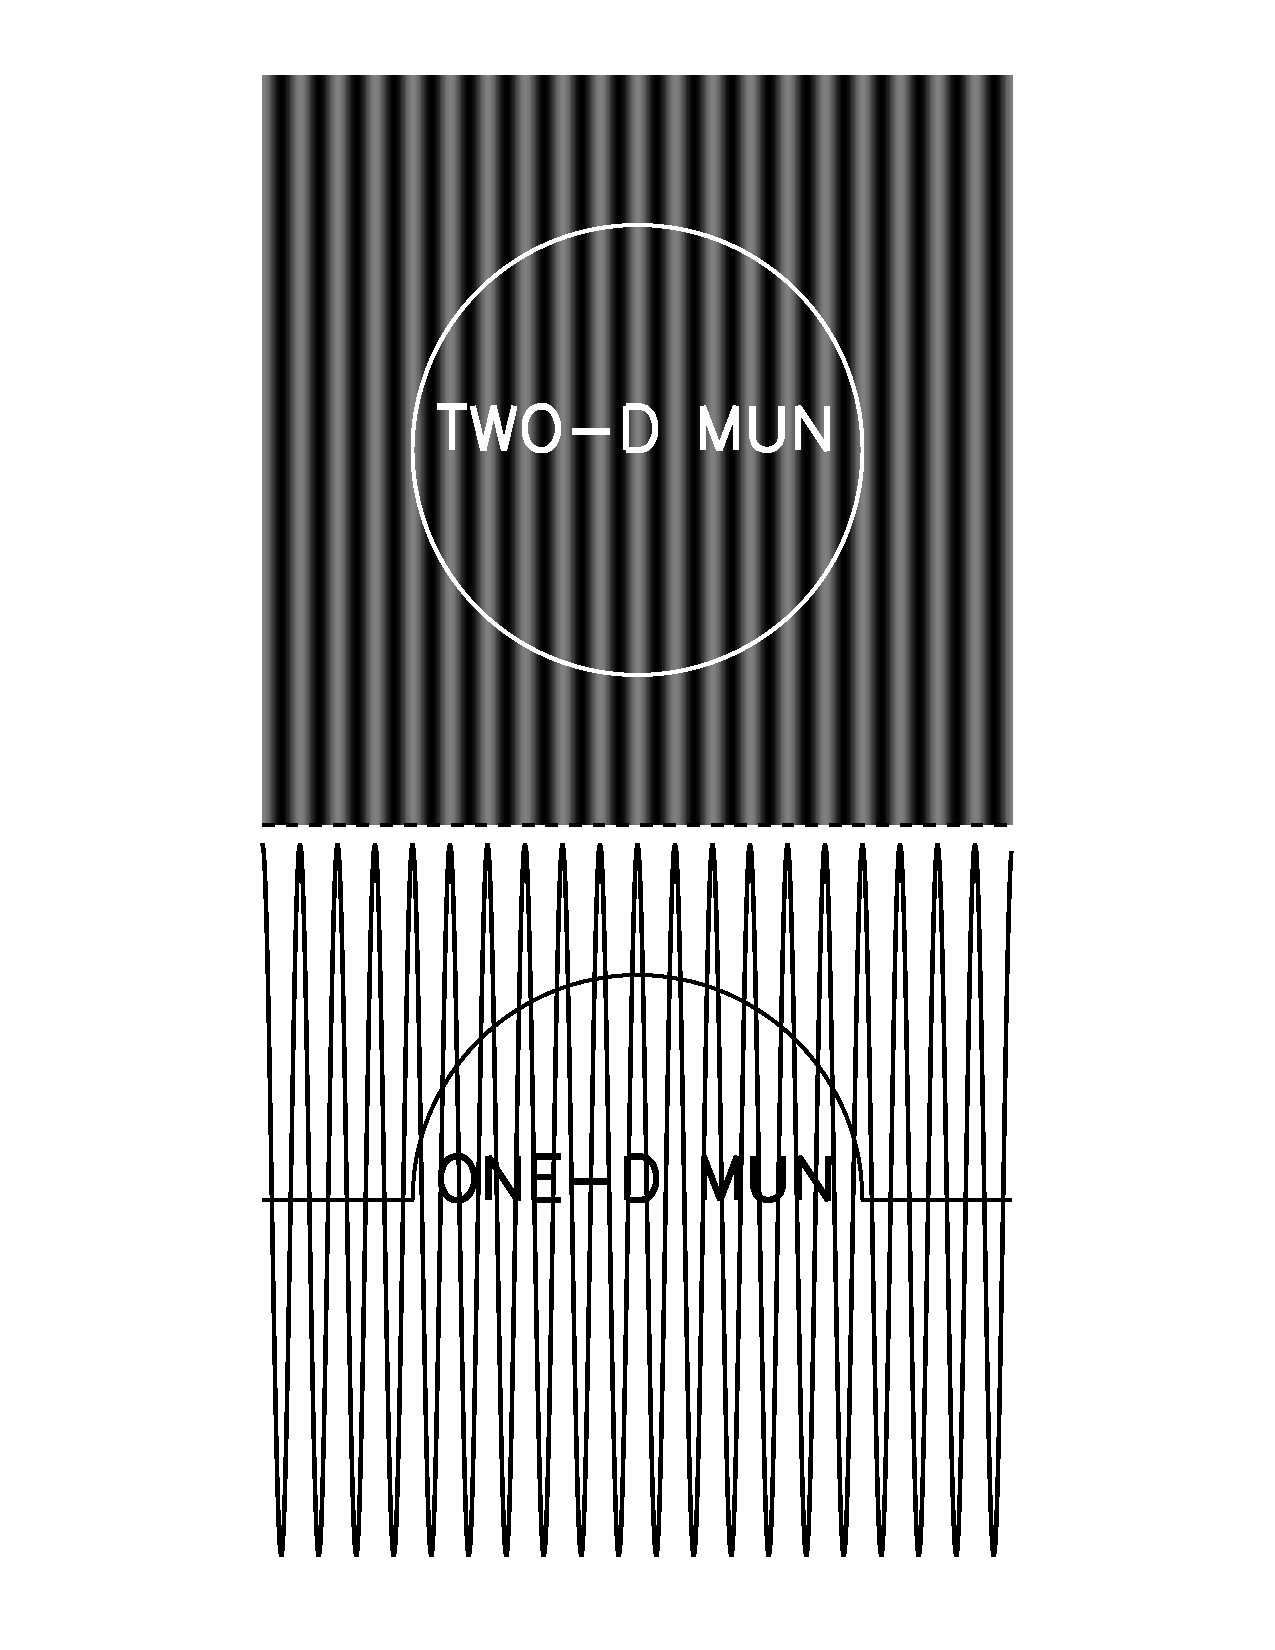
\includegraphics[width=3.0in] {plots/interf_fig.pdf}
\end{center}
                                                                                
\caption{\footnotesize The 2-d and 1-d MUN. At the top, we see the
  situation in the sky as it really is: the fringes cover the 2-d
  object.  At the bottom, we integrate along vertical strips to get the
  1-d brightness distribution and, also, the fringe amplitude (which
  goes from --1 to +1).
\label{interf_fig} } \end{figure}

As the Earth rotates, the source moves through the fringe pattern to
give the fringe response $R(h_s)$. For a point source, $R(h_s)= F(h_s)$
(see equation \ref{maineqn}); for an extended source, we have to
integrate over the extent of the source.  Let $I(h - h_s)$ be the 1-d
intensity distribution in the sky. 
The source center is the intensity-weighted mean of the
position, i.e.

\begin{equation}
h_s = { \int I(h)h dh \over \int I(h) dh} \ .
\end{equation}

\noindent That is, on the bottom panel of
Figure \ref{interf_fig}, $I(h - h_s)$ is the intensity of the source (vertical
direction) and $\Delta h= h -h_s$ the horizontal coordinate---the hour
angle $h$ relative to the hour angle of the source center $h_s$. 


We can express the interferometer response $R(h_s)$ using equation
\ref{maineqn}, which is for a point source; for an extended source, we
imagine $I(\Delta h)$ as being composed of little slices in hour angle,
with each little slice of the source characterized by its position
offset $\Delta h$ and its intensity $I(\Delta h)$, so we just integrate:

\begin{equation} \label{r0a}
R(h_s) = A \int I(\Delta h) \cos \left[ 2\pi \left( {B \over \lambda}
	\cos\delta \right) \sin h\right] d \Delta h +  
	B \int I(\Delta h) \sin\left[ 2\pi \left( {B \over \lambda}
	\cos\delta \right) \sin h \right] \, d \Delta h
\end{equation} 

Now express $\cos \left[ 2\pi \left( {B \over \lambda} \cos\delta
\right) \sin h\right]$ in terms of the local fringe frequency (equations
\ref{taylorexpansion} and \ref{fringefreq}), which replaces $\cos \left[
2\pi \left( {B \over \lambda} \cos\delta \right) \sin h\right]$ by a sum
of two terms, which we temporarily denote $\alpha$ and
$\beta$\footnote{where $\alpha = 2 \pi \left( {B \over \lambda}
\cos\delta \right) \sin{h_s}$ and $\beta = 2 \pi f_f
\Delta h$ .}.  Now, as usual, we use trig identities [$\cos(\alpha +
\beta) = \cos(\alpha) \cos(\beta) - \sin(\alpha) \sin(\beta)$ and
$\sin(\alpha + \beta) = \sin(\alpha) \cos(\beta) + \cos(\alpha)
\sin(\beta)$]. The first (cosine) term of equation \ref{r0a} becomes

\begin{equation}
R^{\cos}(h_s) = A \; \cos(\alpha) \int I(\Delta h) \cos(2\pi f_f \Delta
h) \ d \Delta h 
-A \; \sin(\alpha) \int I(\Delta h) \sin(2\pi f_f \Delta
h) \ d \Delta h 
\end{equation}

\noindent with an equivalent, similar expression for $R^{\sin}(h_s)$.

For our source (the MUN), {\it we assume that $I(\Delta h)$ is
  symmetric} (This also retains our algebraic sanity.). This means that
in the above equation the second term, which is antisymmetric,
integrates to zero.  Similarly, the antisymmetric term in the equivalent
equation $R^{\sin}(h_s)$ also integrates to zero, so we end up with
$R(h_s) = R^{\cos}(h_s) + R^{\sin}(h_s)$, or

\begin{equation} \label{interfeqn}
R(h_s) = \underbrace{ F(h_s)}_{Point-source\ 
Fringe} \times 
\underbrace{\int I(\Delta h) \cos( 2\pi f_f \Delta h) \  d \Delta h}_{Fringe \ Modulator} 
\end{equation}

\noindent Note the structure of equation \ref{interfeqn}. It consists of
two factors. The first ``Point-source Fringe'' term is identical to equation
\ref{fringeresponse}---it's the response to a point source located at
$\Delta h=0$. The other modulates (multiplies) this function. 

Generally, {\it the modulating function is the Fourier transform of the
  source intensity distribution on the sky}.  Here, we assumed a
one-dimensional symmetric source, which means that the sine portion of
the Fourier transform is zero; this is why equation \ref{interfeqn} is
only a cosine Fourier transform instead of a full one.  More generally,
the Fringe Modulator depends on the two-dimensional map of intensity on
the sky, so it's a double integral instead of a single one.  
  
\begin{figure}[h!]
\begin{center}
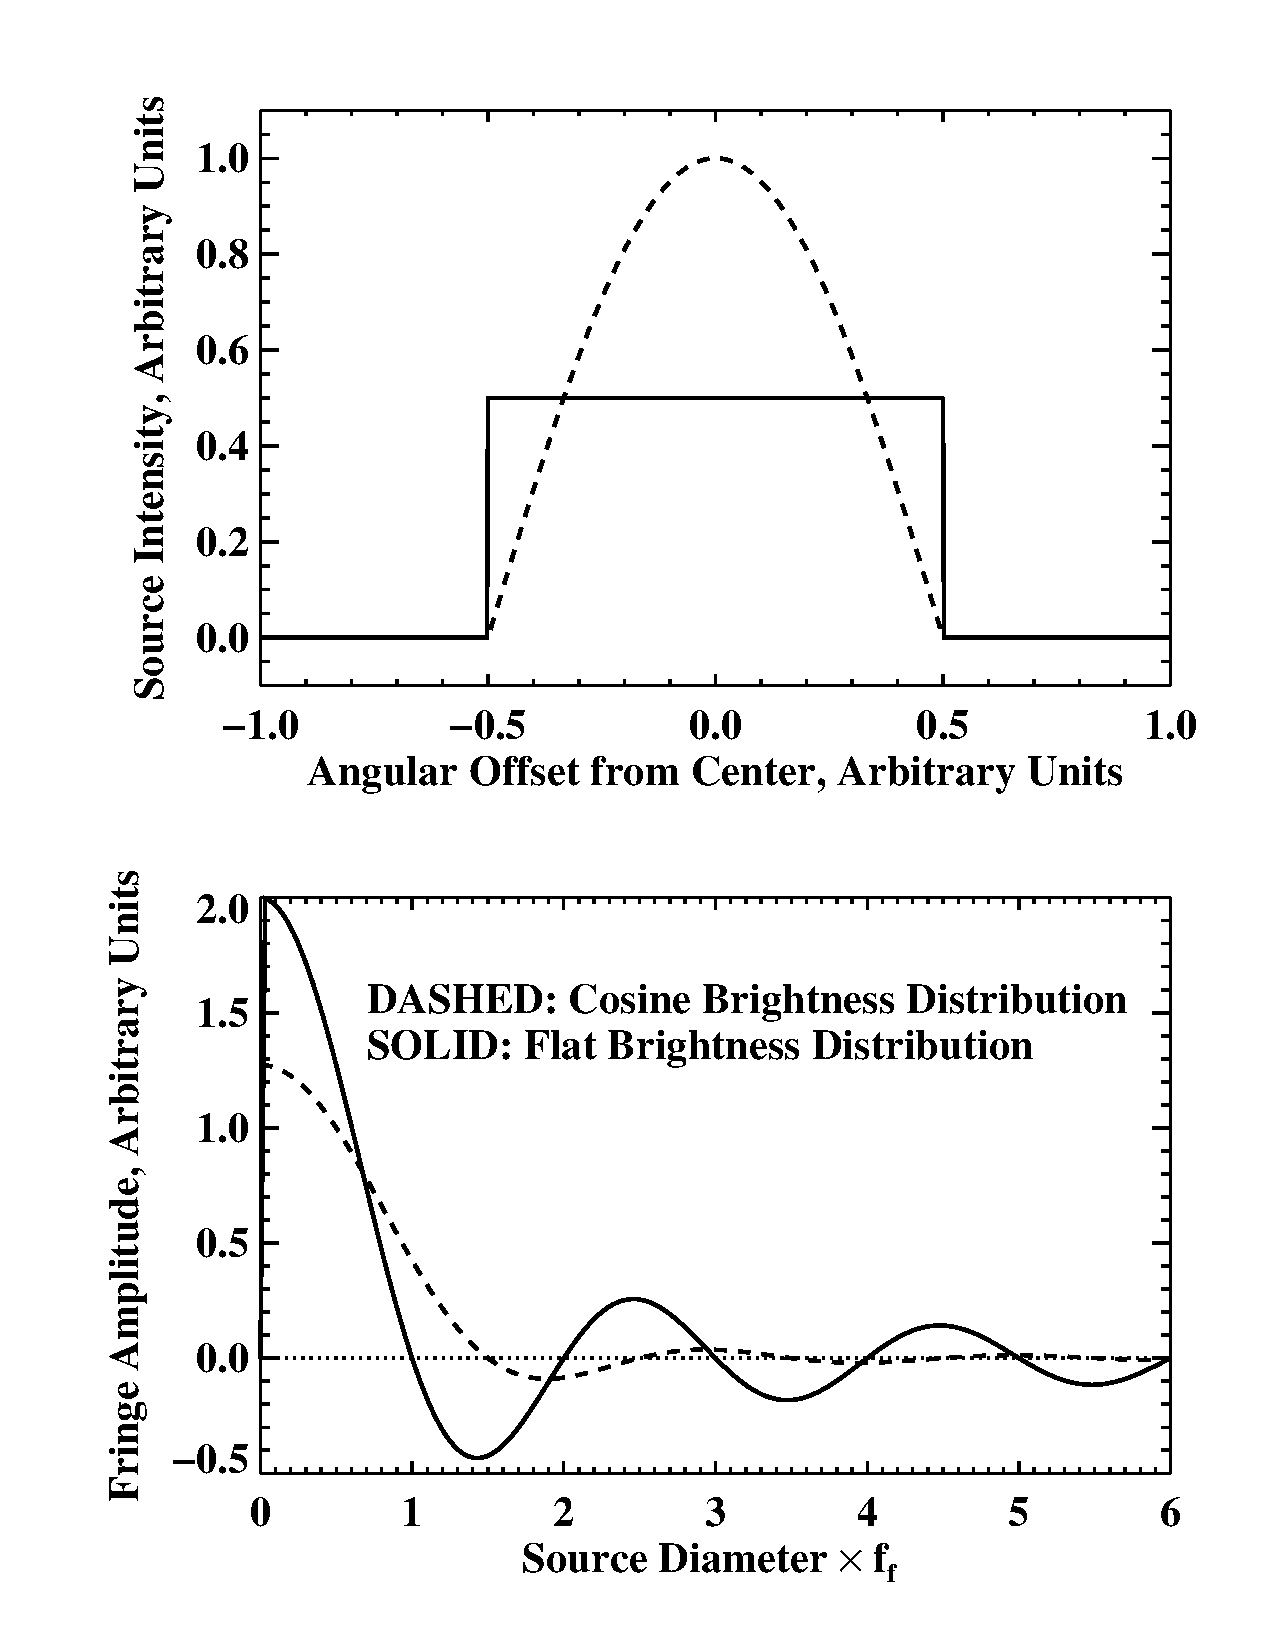
\includegraphics[width=4.0in] {plots/cosfringe.pdf}
\end{center}
                                                                                
\caption{ \footnotesize Examples of 1-d brightness distributions and
  their Fourier transforms. Top panel: the brightness
  distributions. Bottom: the Fourier transforms (Fringe Amplitude
  vs.\ ${Source\ Diameter \over Fringe Period}$). In both, panels, the
  solid line is for a flat brightness distribution and the dashed one
  for a cosine distribution.
\label{cosfringe} } \end{figure}


Figure \ref{cosfringe} (top panel) shows two examples of 1-d brightness
distributions, a flat and a cosine distribution.  The bottom panel shows
the Fourier transforms.  Both of the modulating functions are trig
functions. In particular, for the flat distribution the modulating
function is ${ \sin(2 \pi f_f R) \over 2 \pi f_f R}$. It can (and does!)
go through zero. {\it The locations of these zero points provide crucial
information about the source structure}. The zeros occur for $f_f={n
\over 2R}$. It's more intuitive to express the zeros in terms of fringe
{\it period} (equal to $1 \over f_f$): the zeros occur at $Period = {2R
\over n}$. There's a zero whenever there's an integral number of fringe
periods over the source width. This makes perfect sense, because then
the source contributes equally to the negative and positive portions of
the fringe and the net integral is zero.


\section{MEASURING THE DIAMETER OF A CIRCULAR SOURCE}

\subsection{Theory and Math}
Our goal is to measure and compare the diameters of the Sun and
Moon. We'll make the assumption that the sources are uniformly-bright
disks of radius $R$, which means

\begin{equation}
I(\Delta h) = { (R^2 - \Delta h^2)^{1/2} \over  R}
\end{equation}

\noindent To obtain the theoretical modulating function $MF_{theory}$, you use the integral in
equation \ref{interfeqn}, which is

\begin{equation}
MF_{theory} = {1 \over R} \int_{-R}^R (R^2 - \Delta h^2)^{1/2} 
	\cos(2\pi f_f \Delta h) d \Delta h
\end{equation}

\noindent If you want, you can do this analytically by substituting
$\Delta (R \cos (\theta)$ for $\Delta h$; you end up with a Bessel
function.

We are running a lab class, not a math class, so let's proceed by doing
the integral {\it numerically}! To accomplish this, split $I(\Delta h)$
into $2N + 1$ tiny little slices (the total number is odd, which makes
the slices symmetric about $\Delta h = 0$). Each slice has width $\delta
h = {R \over N}$, and $\Delta h_n = n \delta h$, where $n$ runs from
$-N$ to $+N$. Then the integral becomes a sum:

\begin{equation}
MF_{theory} \approx {1 \over R} \sum_{n=-N}^{n=+N}
[R^2 - (n \delta h)^2]^{1/2} \cos(2 \pi f_f n\delta h) \delta h
\end{equation}

\noindent which we rewrite as

\begin{equation}
MF_{theory} \approx  \delta h \sum_{n=-N}^{n=+N}
\left[ 1 - \left( n \over N\right)^2 \right]^{1/2} 
\cos \left( 2 \pi f_f R n \over N \right)
\end{equation}

\subsection{Important Mathematical and <<<PRACTICAL!!! Point!}

Note the {\it first important point} that $MF_{theory}$\dots \begin{itemize}
\item is a function {\it only} of the combination $f_f R$, and
\item in particular, has zero crossings that occur at specific
  values of $f_f R$.
  \end{itemize}

  Note the {\it second important point} that for $MF_{observed}$\dots
  \begin{itemize}
    \item The zero crossings occur at specific measured values of
      $f_{f}$. \end{itemize} 

\noindent Thus, by comparing the zero crossing numbers for $MF_{theory}$ and
$MF_{observed}$, you get the radius $R$. 


\section {REFERENCE READING on INTERFEROMETRY AND APERTURE SYNTHESIS}

	The appropriate reference for our purposes is the article {\it
Interferometry and Aperture Synthesis}, which is chapter 10 of the book
{\it Galactic and Extragalactic Radio Astronomy, First Edition}.  The
authors are Fomalont and Wright; Melvyn Wright is a research scientist
in our radio lab here at Berkeley and is a real expert.  This chapter is
excellent, providing the basics without excessive detail (although it
has more than we need).  If you want more depth than we provide here, we
suggest the following sections of this chapter: {\bf (1)} \S10.1.3,
which describes a two-element interferometer; section {\it e} of this
chapter is on polarization and you can skip it; {\bf (2)} \S10.2.1 and
\S10.2.2, which describe ``a working interferometer''; and {\bf (3)}
Appendix II, which describes the geometrical details. 

	There is a scaling mistake in their equation for the fringe
frequency $\nu_f$: their equation needs to be multiplied by the rotation
rate of the Earth in radians per second.  For example, for an east-west
baseline of 343.8 wavelengths looking at declination zero on the
meridian, the fringe frequency on the sky is 343.8 fringes per radian. 
This means that the fringe spacing on the sky is ${1 \over 343.8}$
radians or 10 arcmin; it takes the Earth 40 seconds of time to turn
through 10 arcmin, so the fringe period in this case is 40 seconds and
$\nu_f = .025$ Hz.  More generally, for this east-west interferometer
the fringe frequency is $\nu_f = .025 \cos \delta \cos h$ Hz, where
$\delta$ is the declination and $h$ the hour angle. 

	If you want to know really everything and in complete
mathematical detail, read the book {\it Interferometry and Synthesis in
Radio Astronomy} by Thompson, Moran, and Swenson.  But such detail is
more than we want and can be overwhelming.  Our main interest is the
geometry---how the baseline projects on the $u-v$ plane.  This is in
chapter 4, and the most important sections for us are chapter 4.2 and
4.4. 

With the longer baselines of research-class interferometers/arrays comes
increased angular resolution, and all of our sources become finite in
angular size, which means that the telescope arrays can map the sources
using Fourier techniques. Some types of source are so small that mapping
them requires interferometers with baseline lengths comparable to the
Earth's diameter, a technique called ``Very Long Baseline
Interferometry'' (VLBI). And some sources, such as pulsars, are even too
small for VLBI!


\end{document}

3C144 (Crab Nebula) & $05^h31^m30^s$ & $21^\circ 58'$
                    & $05^h34^m23^s$ & $22^\circ 00'$ & $\sim 496$ \cr
Orion Nebula        & $05^h32^m44^s$ & $-05^\circ 25'$
                    & $05^h35^m05^s$ & $-05^\circ 23'$ & $\sim 340$ \cr
3C274 (Virgo A)     & $12^h28^m18^s$ & $12^\circ 40'$
                    & $12^h30^m44^s$ & $12^\circ 24'$ & $\sim 34$ \cr
M17                 & $18^h17^m33^s$ & $-16^\circ 12'$
                    & $18^h20^m19^s$ & $-16^\circ 11'$ & $\sim 500$ \cr
3C405 (Cygnus A)    & $19^h57^m45^s$ & $40^\circ 36'$
                    & $19^h59^m24^s$ & $40^\circ 44'$ & $\sim 120$ \cr  
3C461 (Cas A)       & $23^h21^m07^s$ & $58^\circ 34'$
                    & $23^h23^m17^s$ & $58^\circ 50'$ & $\sim 320$ \cr 
SUN                 &   varies       &   varies \cr
MOON                &   varies       &   varies \cr

*************************
-------------

Now write $U = \left( {B_y \over \lambda} \cos\delta \right)$ ($U$ is
the east-west projected baseline expressed in
wavelenths)\footnote{Conventionally, the letters $[U,\, V,\, W]$ represent
  the projection of the baseline in the EW, NS, and vertical directions,
  respectively.} and use
equation \ref {fringeresponse} to write

\begin{equation} \label{r0}
R(h_s) = A \int I(h-h_s) \cos( 2\pi U \sin h) \ dh +  
	B \int I(h-h_s) \sin( 2\pi U \sin h) \ dh
\end{equation} 

	Our source occupies a small angle, so we can expand $h$ around $h_s$
by writing $[\Delta h = h-h_s]$. We use equation \ref{taylorexpansion} to
expand $\sin h$ as $\sin h \approx \sin( h_s) + \Delta h \cos( h_s)$.
Things are getting algebraically cumbersome, so let's eliminate
clutter by defining 

\begin{mathletters}
\begin{equation}
\alpha(h_s) = 2 \pi U \sin(h_s) 
\end{equation}
\begin{equation}
\beta(h_s, \Delta h) = 2 \pi U \cos(h_s) \  \Delta h = 2 \pi f_f \Delta h
\end{equation}
\end{mathletters}

\noindent [where $U = \left( {B \over \lambda} \cos\delta \right)$] so that equation \ref{r0} becomes

\begin{equation} \label{r1}
R(h_s) = A \int I(h-h_s) \cos( \alpha + \beta) \ dh +  
	B \int I(h-h_s) \sin( \alpha + \beta) \ dh
\end{equation} 

\noindent Now, as usual, we use trig identities [$\cos(\alpha + \beta) =
  \cos(\alpha) \cos(\beta) - \sin(\alpha) \sin(\beta)$ and $\sin(\alpha
  + \beta) = \sin(\alpha) \cos(\beta) + \cos(\alpha) \sin(\beta)$]. The
  first (cosine) term of equation \ref{r1} becomes

\begin{equation}
R^{\cos}(h_s) = A \; \cos(\alpha) \int I(\Delta h) \cos( \beta) \ d \Delta h 
-A \; \sin(\alpha) \int I(\Delta h) \sin( \beta) \ d \Delta h 
\end{equation}

\noindent with an equivalent, similar expression for $R^{\sin}(h_s)$. We
imagine $I(\Delta h)$ as being composed of little slices in hour angle,
with each little slice of the source characterized by its position
offset $\Delta h$ and its intensity $I(\Delta h)$. 
*****************************

\begin{equation} \label{interfeqn}
R(h_s) = 
\underbrace{ \left\{ A \; \cos[\alpha(h_s)]
\ + B \; \sin[\alpha(h_s)]
\right\}}_{Point-source\ 
Fringe} \times 
\underbrace{\int I(\Delta h) \cos[ \beta(h_s,\Delta h)] \ d \Delta h}_{Fringe \ Modulator} 
\end{equation}

Now at any one time (hour angle $h_s$) the fringe pattern in the
vicinity of the source is a sine wave with frequency $f_f(h_s)$ cycles
per radian and has the functional form $F(f_f,\Delta h) = [A' \cos( 2
\pi f_f \Delta h) + \sin( 2 \pi f_f \Delta h)]$, where $A'$ and $B'$ are
constants that tell the fringe amplitude and phase with respect to
$\Delta h = 0$, i.e.\ with respect to $h_s$.  $F(f_f,\Delta h)$ covers
the source with fringes of angular frequency $f_f$, and the
interferometer response $R(h_s)$ is the integral of this local fringe
pattern times the source intensity distribution, so we have

\begin{equation}
R(h_s) = \int F(f_f,\Delta h) I(\Delta h) \ d \Delta h
\end{equation}

\noindent (Recall $f_f(h_s)$ depends on $h_s$, so $R$ is a function of $h_s$.)
This equation is physically intuitive because it expresses the fringe
response at any particular hour angle as depending on the fringe
frequency and the source structure; the source is small, so it covers a
small range of hour angle, i.e.\ a small range of $\Delta h$. 

